\documentclass{beamer}

\usetheme{Singapore}

\usepackage{graphicx}
\usepackage{listings}


\lstset{basicstyle=\small\ttfamily,
  numbers=left,
  escapeinside=||
}

\usepackage{color}

\definecolor{dkgreen}{rgb}{0,0.6,0}
\definecolor{gray}{rgb}{0.5,0.5,0.5}
\definecolor{mauve}{rgb}{0.58,0,0.82}

\lstset{frame=tb,
  language=Python,
  aboveskip=3mm,
  belowskip=3mm,
  showstringspaces=false,
  columns=flexible,
  basicstyle={\small\ttfamily},
  numbers=none,
  numberstyle=\tiny\color{gray},
  keywordstyle=\color{blue},
  commentstyle=\color{dkgreen},
  stringstyle=\color{mauve},
  breaklines=true,
  breakatwhitespace=true,
  tabsize=3
}

%==========================(Casey's LaTeX Shortcuts)================================
%===================================================================================

% SYMBOLS %
% ---------------------- Blackboard Bold --------------------------------
\def\R{\mathbb{R}}                     % real numbers R
\def\C{\mathbb{C}}                     % complex numbers C
\def\N{\mathbb{N}}                     % natural numbers
\def\Z{\mathbb{Z}}                     % integers
\def\Q{\mathbb{Q}}                     % rational numbers
\def\P{\mathbb{P}}                     % primes
\def\W{\mathbb{W}}                     % windowing functions
\def\B{\mathbb{B}}                     % partition of unity functions
\def\A{\mathbb{A}}                     % almost orthogonal windowing functions
\def\T{\mathbb{T}}                     % unit circle (\R mod 2 \pi)
\def\F{\mathbb{F}}                     % Functions
\def\I{\mathbb{I}}                     % Intervals
\def\D{\mathbb{D}}                     % The unit disk
\def\Rn{{\R}^{n}}                      % n-dimensional R space
\def\Cn{{\C}^{n}}                      % n-dimensional C space
\def\Rhat{{\widehat{\R}}}              % reals (dual)
\def\Rnhat{{\widehat{\Rn}}}            % n-dim reals (dual)
\def\PW{\mathbb{PW}}                   % Paley-Wiener Space

% WORD FUNCTIONS %
\def\sinc{\mathop{\textstyle{\rm sinc}}}
\def\domain{\mathop{\textstyle{\rm Domain}}\nolimits}
\def\essinf{\mathop{\textstyle{\rm ess \, inf}}}
\def\esssup{\mathop{\textstyle{\rm ess \, sup}}}
\def\range{\mathop{\textstyle{\rm Range}}\nolimits}
\def\Span{\mathop{\textstyle{\rm span}}\nolimits}
\def\supp{\mathop{\textstyle{\rm supp}}\nolimits}
\def\CHI{\hbox{\raise .5ex \hbox{$\chi$}}}
\def\Tri{\mbox{Tri}}
\def\Trap{\mbox{Trap}}
\def\Cap{\mbox{Cap}}
\def\loc{{\textstyle{\rm loc}}}
\def\qed{ \hspace*{\fill} \Box}

% UNARY, BINARY OPERATORS %
\def\norm#1{\|  #1 \|}
\def\abs#1{| #1 |}
\def\bigabs#1{\biggl| #1 \biggr|}
\def\set#1{\{ #1 \}}
\def\bigset#1{\biggl\{ #1 \biggr\}}
\def\ceiling#1{\lceil #1 \rceil}
\def\floor#1{\lfloor #1 \rfloor}
\def\ip#1#2{\langle #1 , #2 \rangle}
\def\bigip#1#2{\bigl\langle #1, \, #2 \bigr\rangle}
\def\Bigip#1#2{\Bigl\langle #1, \; #2 \Bigr\rangle}
\def\biggip#1#2{\biggl\langle #1, \; #2 \biggr\rangle}
\def\ipsize#1#2{\left\langle #1 , #2 \right\rangle}
\def\Int#1{\lfloor #1 \rfloor}
\def\biggInt#1{\biggl\lfloor #1 \biggr\rfloor}
\def\Intsize#1{\left\lfloor #1 \right\rfloor}
\def\paren#1{( #1 )}
\def\bigparen#1{\left( #1 \right)}
\def\Bigparen#1{\Bigl( #1 \Bigr)}
\def\biggparen#1{\biggl( #1 \biggr)}
\def\Biggparen#1{\Biggl( #1 \Biggr)}
\def\sqparen#1{[ #1 ]}
\def\bigsqparen#1{\biggl[ #1 \biggr]}

\newcommand{\hl}[1]{{\bf #1}}
\newcommand{\refp}[1]{(\ref{#1})}

\def\comment#1{}

%==========================(End of my LaTeX Commands)===============================
%

%\begin{document}

\title{
{\bf{\textsf{Hack the Derivative!}}}}
\author[Erik Taubeneck]{Erik Taubeneck}

\institute{
  GameChanger Media - Software Engineer

  We're hiring! \url{https://gc.com/about/careers}
}

\date{August 15th, 2015}

\begin{document}

% Creates title page of slide show using above information


\begin{frame}
  \titlepage
\end{frame}

%\section[Outline]{}

\begin{frame}
\frametitle{Outline}
\tableofcontents
\end{frame}

\begin{frame}[fragile]

  \frametitle{Try It Yourself}

  The functions used through out this presentations can be installed with pip!

  \begin{lstlisting}
      $ mkdir somewhere_new
      $ cd somewhere_new
      $ virtualenv venv
      $ source venv/bin/activate
      $ pip install hackthederivative
      $ python
      >>> from hackthederivative import *
  \end{lstlisting}

\end{frame}


\section{Calculus Crash Course}

\begin{frame}

  \frametitle{Taking the Derivative}

  Let $f(x)$ be a function from $\R \to X \subseteq \R$.

  e.g.
  \begin{itemize}
    \item $f(x) = x^2$
    \item $g(x) = sin(x)$
    \item $h(x) = 5x^3 - 6x + \frac{1}{x}$ \footnote{Note that $h(x)$ is not defined at $x=0$.}
  \end{itemize}



\end{frame}

\begin{frame}

  \frametitle{Taking the Derivative}

  The derivative of $f(x)$, $f'(x)$, is a new function which tells us the \textit{slope} of the tangent line that intersects $f$ at any given $x$.

  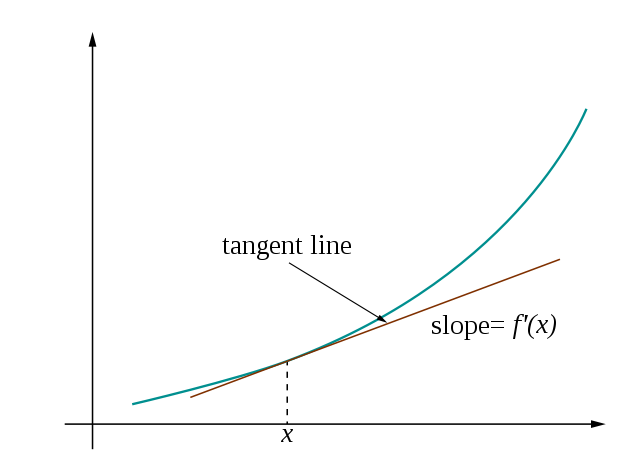
\includegraphics[scale=.4]{tangent.png}

\end{frame}

\begin{frame}

  \frametitle{Taking the Derivative}

  Formally, the derivative of $f(x)$ at $x$ is

  \[ f'(x) = \lim_{h \to 0} \frac{f(x+h) - f(x)}{h} \]

\end{frame}

\begin{frame}

  \frametitle{Taking the Derivative}

  $\mathbb{E}^x$:

  Let $f(x) = x^2$. \pause Then

  \begin{eqnarray*}
    f'(x) &&  = \lim_{h \to 0} \frac{(x+h)^2 - x^2}{h} \\ \pause
    && = \lim_{h \to 0} \frac{x^2 + 2xh + h^2 - x^2}{h} \\ \pause
    && = \lim_{h \to 0} \frac{2xh + h^2}{h} \\ \pause
    && = \lim_{h \to 0} 2x + h \\ \pause
    && = 2x \\
  \end{eqnarray*}

  $\qed$

\end{frame}

\section{Finite Difference}

\begin{frame}
\frametitle{Finite Difference}

Suppose we wish to find the derivative for some function $f(x)$ a $x_0$.

\pause
One approximation is the finite difference method.

\pause
Recall

\[ f'(x) = \lim_{h \to 0} \frac{f(x+h)-f(x)}{h} \]

\pause
We can estimate

\[ f'(x_o) \approx \frac{f(x_0+h)-f(x_0)}{h} \]

for some small $h$.



\end{frame}

\begin{frame}[fragile]
\frametitle{Finite Difference}

Implemented in Python

\begin{lstlisting}
  In [1]: def finite_difference(f, x, h):
              return (f(x+h) - f(x))/h
  |\pause|
  In [2]: f = lambda x: x**2

  In [2]: finite_difference(f, 1.0, 0.00001)

  Out [3]: 2.00001000001393
\end{lstlisting}

\end{frame}

\begin{frame}[fragile]
\frametitle{Finite Difference}

But how do we choose $h$? \pause

The limit as $h \to 0$ approaches the derivative, so the smaller the better!

\begin{lstlisting}
  In [4]: import sys

  In [5]: h = sys.float_info.min
  |\pause|
  In [6]: print finite_difference(f, 1.0, h)

  Out [6]: 0.0
\end{lstlisting}


Uh oh.

\end{frame}

\begin{frame}[fragile]
\frametitle{Finite Difference}

Hmm, $0.00001$ seems pretty small, and worked well earlier.

Maybe that will just work.

\pause

\begin{lstlisting}
  In [7]: finite_difference(f, 1.0e20, 0.00001)

  Out [7]: 0.0
\end{lstlisting}

Nope, that can break too.

To figure out why, let's look closer at Floating Point numbers.

\end{frame}

\section{Floating Point Arithmetic}


\begin{frame}

\frametitle{Floating Point Numbers}

A Float64, or a double-precision floating-point number, consists of

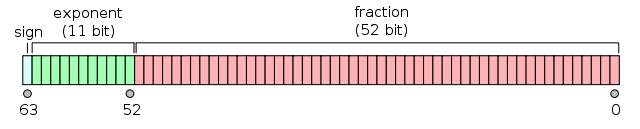
\includegraphics[scale=.4]{float-format.png}

and represents the real number $x \in \R$ with $sign$, $e$, and $b_i$ such that

\[ (-1)^{sign} (1.b_{51}b_{50}...b_{0})_2 \ 2^{e-1023} \]

or (possibly more readable)

\[ (-1)^{sign} \left ( 1 + \sum_{i=1}^{52} b_{52-i} 2^{-i} \right ) \times 2^{e-1023} \]

\end{frame}

\begin{frame}

\frametitle{Floating Point Numbers}

Multiplication is helped by Associativity and Commutativity

\begin{eqnarray*}
     && (5.916829373 \times 10^{23}) \times (7.208209342 \times 10^{-51}) \\ \pause
  =  && 5.916829373 \times 10^{23} \times 7.208209342 \times 10^{-51} \\ \pause
  =  && 5.916829373 \times 7.208209342 \times 10^{23} \times 10^{-51} \\ \pause
  =  && (5.916829373 \times 7.208209342) \times (10^{23} \times 10^{-51}) \\ \pause
\end{eqnarray*}

but this doesn't work for addition \pause

\begin{eqnarray*}
      && (5.916829373 \times 10^{23}) + (7.208209342 \times 10^{-51}) \\
\end{eqnarray*}

\end{frame}

\begin{frame}

\frametitle{Floating Point Numbers}

This means that the floating point numbers have gaps!

\begin{center}
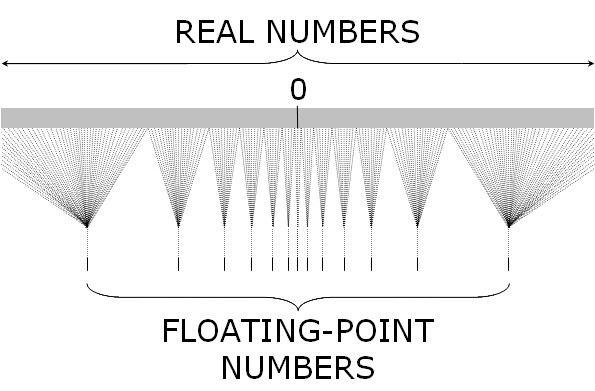
\includegraphics[scale=.6]{float-gaps.jpg}
\end{center}

\end{frame}



\begin{frame}[fragile]
\frametitle{Floating Point Gaps}

\begin{lstlisting}

  In [1]: import sys

  In [2]: plus_epsilon_identity(x, eps):
              return x + eps == x

  In [3]: eps = sys.float_info.min
  |\pause|
  In [4]: plus_epsilon_identity(0.0, eps)
  Out [4]: False

  In [5]: plus_epsilon_identity(1.0, eps)
  Out [5]: True
  |\pause|
  In [6]: plus_epsilon_identity(1.0e20, 1.0)
  Out [6]: True

\end{lstlisting}

\end{frame}

\begin{frame}
\frametitle{Problems with the Derivative}

If we choose $h$ that is so small such that

\[ float(x) + float(h) = float(x) \]
\pause

then

\[ \frac{f(x+h) - f(x)}{h} = \frac{f(x) - f(x)}{h} = \frac{0}{h} = 0 \]

\end{frame}


\begin{frame}[fragile]
\frametitle{Choosing Epsilon}

\begin{lstlisting}

  In [1]: def eps(x):
              e = float(max(sys.float_info.min, abs(x)))
              while not plus_epsilon_identity(x, e):
                  last = e
                  e = e / 2.
              return last
  |\pause|
  In [2]: eps(1.0)
  Out[2]: 2.220446049250313e-16

  In [3]: eps(1.0e10)
  Out[3]: 1.1102230246251565e-06
  |\pause|
  In [4]: eps(1.0e20)
  Out[4]: 11102.230246251565
\end{lstlisting}

\end{frame}

\begin{frame}[fragile]
\frametitle{Choosing Epsilon}

From \href{http://www.karenkopecky.net/Teaching/eco613614/Notes_NumericalDifferentiation.pdf}{lecture notes posted by Karen Kopecky} \footnote{\url{http://www.karenkopecky.net/Teaching/eco613614/Notes_NumericalDifferentiation.pdf}}, we see we should use

\[ h = \sqrt{u} * max(\abs{x}, 1) \]

where $u = eps(1)$.
\pause
\begin{lstlisting}

  In [1]: def finite_difference(f, x, h=None):
              if not h:
                  h = sqrt(eps(1.0)) * max(abs(x), 1.0)
              return (f(x+h) - f(x))/h

\end{lstlisting}

\end{frame}

\begin{frame}[fragile]
\frametitle{Testing It Out}

\begin{lstlisting}

  In [2]: def error(f, df, x):
              return abs(finite_difference(f, x) - df(x))

  In [3]: def error_rate(f, df, x):
              return error(f, df, x) / df(x)
  |\pause|
  In [4]: f, df = lambda x:x**2, lambda x:2*x
  |\pause|
  In [5]: error_rate(f, df, 1.0)
  Out[5]: 7.450580596923828e-09
  |\pause|
  In [6]: error_rate(f, df, 1.0e5)
  Out[6]: 9.045761108398438e-09
  |\pause|
  In [7]: error_rate(f, df, 1.0e20)
  Out[7]: 4.5369065472e-09
\end{lstlisting}

\end{frame}

\begin{frame}[fragile]
\frametitle{Testing It Out}

\begin{lstlisting}

  In [8]: import math

  In [9]: f, df = math.sin, math.cos
  |\pause|
  In [10]: error_rate(f, df, 1.0)
  Out[10]: 1.2780011808656197e-08
  |\pause|
  In [11]: error_rate(f, df, 1.0e10)
  Out[11]: 1.002014830004253
  |\pause|
  In [12]: error_rate(f, df, 1.0e20)
  Out[12]: 0.9999999999998509
\end{lstlisting}

\end{frame}

\begin{frame}
\frametitle{We Can Do Better!}
\pause
\begin{center}
  
\includegraphics[scale=0.5]{use-math.png}
\end{center}

\end{frame}

\section{Complex Analysis Crash Course}

\begin{frame}
\frametitle{A Crash Course in Complex Analysis}

\begin{itemize}[<+->]
  \item Def: $i$ = $\sqrt{-1}$.
  \item Why do we need $i$???
  \item Solve $x^2 + 1 = 0$
  \item Def: $\C = \{x + iy \ \forall \ x,y \ \in \R^2 \}$
  \item Fun fact! All polynomials of degree $n$ have $n$ zeros in $\C$.
\end{itemize}


\end{frame}

\begin{frame}
\frametitle{A Crash Course in Complex Analysis}

$\mathbb{E}^x$:
\[ f(z) = z^2 \]
\pause
Let $z=x+iy$. Then
\[ f(z) = f(x+iy) = (x+iy)^2 = x^2 +2ixy + i^2y^2 = \]
\[ x^2+ 2ixy - y^2 \]

\pause
We can always write $f(x+iy) = u(x,y) + iv(x,y)$. Note that

\[ u(x,y) = \mathfrak{R}(f(x+iy)) \ \mathrm{and} \ v(x,y) = \mathfrak{I}(f(x+iy)) \]

\pause
In our example
\[ u(x,y) = x^2 - y^2 \ \mathrm{and} \ v(x,y) = 2xy \]

\end{frame}

\begin{frame}
\frametitle{A Crash Course in Complex Analysis}

\[ u(x,y) = x^2 - y^2 \ \mathrm{and} \ v(x,y) = 2xy \]

We can now take 4 different derivatives.

\begin{eqnarray*}
\frac{\partial u}{\partial x} = 2x && \frac{\partial v}{\partial x} = 2y \\
\frac{\partial u}{\partial y} = -2y && \frac{\partial v}{\partial y} = 2x
\end{eqnarray*}

\pause
  Note that:
  \begin{eqnarray*}
  \frac{\partial u}{\partial x} = \frac{\partial v}{\partial y} &&
  \frac{\partial u}{\partial y} = -\frac{\partial v}{\partial x}
  \end{eqnarray*}

\end{frame}

\begin{frame}
\frametitle{Cauchy-Riemann Equations}
  These are the Cauchy-Riemann equations and hold for all analytic functions on $\C$! \footnote{See your favorite Complex Analysis textbook for a proof.}
  \begin{eqnarray*}
  \frac{\partial u}{\partial x} = \frac{\partial v}{\partial y} &&
  \frac{\partial u}{\partial y} = -\frac{\partial v}{\partial x}
  \end{eqnarray*}



\end{frame}


\section{Hack the Derivative}
\begin{frame}
\frametitle{Time for the Hack!}

  We have $f:\R \to X \subseteq \R$. Rewrite
  \[ f(z) = f(x+iy) = u(x,y) + iv(x,y) \]
  \pause
  Now, for all $\bar{z} \in \R$, we have $y = 0$, and so
  \[ f(\bar{z}) = f(x,0) = u(x,0) + iv(x,0) \]
  \pause
  Since $f: \R \to X \subseteq \R$, $f(\bar{z}) \in \R$ for all $\bar{z} \in \R$. Therefore
  \[ v(x,0) = 0 \]
  \pause
  and so
  \[ f(x,0) = u(x,0) \]
  \pause
  We want to estimate $\frac{df}{\partial x}$. Since for all $z \in \R$, $f = u$,
  \[ \frac{df}{\partial x} = \frac{\partial u}{\partial x} = \frac{\partial v}{\partial y} \]

\end{frame}

\begin{frame}
\frametitle{Time for the Hack!}

  Again, using the definition of the derivative
  \[ \frac{\partial v}{\partial y} = \lim_{h \to 0} \frac{v(x,y+h) - v(x,y)}{h} \]
  \pause
  Since $y = 0$ for all $\bar{z} \in \R$,
  \[ \frac{\partial v}{\partial y} = \lim_{h \to 0} \frac{v(x,h) - v(x,0)}{h} \]
  \pause
  Recall that $v(x,0) = 0$, so
  \[ \frac{\partial v}{\partial y} = \lim_{h \to 0} \frac{v(x,h)}{h} \]
  \pause
  Now, to estimate $\frac{df}{\partial x} = \frac{\partial v}{\partial y}$, for a very small $h$
  \[ \frac{df}{\partial x} \approx \frac{v(x,h)}{h} = \frac{\mathfrak{Im}(f(x+ih))}{h} \]


\end{frame}

\begin{frame}[fragile]
\frametitle{Complex Step Finite Difference}

Implemented in Python


\begin{lstlisting}
  In [1]: import sys

  In [2]: def complex_step_finite_diff(f, x):
              h = sys.float_info.min
              return (f(x+h*1.0j)).imag / h
\end{lstlisting}
\end{frame}

\begin{frame}[fragile]
\frametitle{Complex Step Finite Difference}

Implemented in Python


\begin{lstlisting}
  In [3]: f, df = lambda x:x**2, lambda x:2*x
  |\pause|
  In [4]: complex_step_finite_diff(f, 1.0)
  Out[4]: 2.0
  |\pause|
  In [5]: complex_step_finite_diff(f, 1.0e10)
  Out[5]: 20000000000.0
  |\pause|
  In [6]: complex_step_finite_diff(f, 1.0e20)
  Out[6]: 2e+20


\end{lstlisting}
\end{frame}

\begin{frame}[fragile]
\frametitle{Testing It Out}

\begin{lstlisting}

  In [7]: def cerror(f, df, x):
              return abs(complex_step_finite_diff(f, x) - df(x))

  In [8]: def cerror_rate(f, df, x):
              return cerror(f, df, x) / x
  |\pause|
  In [9]: cerror_rate(f, df, 1.0)
  Out[9]: 0.0   |\pause|
  In [10]: cerror_rate(f, df, 1.0e10)
  Out[10]: 0.0   |\pause|
  In [11]: cerror_rate(f, df, 1.0e20)
  Out[11]: 0.0   |\pause|
\end{lstlisting}

\end{frame}

\begin{frame}[fragile]
\frametitle{Testing It Out}

\begin{lstlisting}

  In [11]: import cmath

  In [11]: f, df = cmath.sin, cmath.cos
  |\pause|
  In [12]: cerror_rate(f, df, 1.0)
  Out[12]: 0.0
  |\pause|
  In [13]: cerror_rate(f, df, 1.0e10)
  Out[13]: 0.0
  |\pause|
  In [14]: cerror_rate(f, df, 1.0e20)
  Out[14]: 0.0
\end{lstlisting}

\end{frame}

\begin{frame}[fragile]
\frametitle{It's Not Perfect, But It's Pretty Good}

\begin{lstlisting}

  In [15]: cerror_rate(f, df, 1.0e5)
  Out[15]: .110933124815182e-16
  |\pause|
  In [16]: f = lambda x: cmath.exp(x) / cmath.sqrt(x)
  In [17]: df = lambda x: (cmath.exp(x)* (2*x - 1))/(2*x**(1.5))
  |\pause|
  In [18]: cerror_rate(f, df, 1.0)
  Out[18]: 0.0   |\pause|
  In [19]: cerror_rate(f, df, 1.0e2)
  Out[19]: 1.1570932160552342e-16   |\pause|
  In [20]: cerror_rate(f, df, 5.67)
  Out[20]: 1.2795419601231268e-16   |\pause|
  In [21]: cerror_rate(f, df, 1.0e3)
  Out [21]: OverflowError: math range error

\end{lstlisting}

\end{frame}


\begin{frame}
\frametitle{Limits}

  \begin{itemize}
    \item Must satisfy Cauchy Riemann equations, so does not work for abs or a function with $<$ or $>$ in it.
    \item Only works for functions from $\R \to X \subseteq \R$.
  \end{itemize}

\end{frame}

\begin{frame}

\frametitle{Thanks!}

\begin{itemize}
  \item Follow me on twitter: \href{https://twitter.com/taubeneck}{@taubeneck}
  \item Fork me on Github: \href{https://github.com/eriktaubeneck}{eriktaubeneck}
  \item Blog: \url{http://skien.cc/}
  \item Slides: \url{http://slides.skien.cc/hack-the-derivative-pygotham.pdf}
  \item Other Presentations: \url{http://slides.skienc.cc}
\end{itemize}

\end{frame}

\end{document}
